\documentclass[12pt, a4paper, titlepage]{article}
\usepackage[utf8]{inputenc}

\usepackage{amsmath}
\usepackage{amssymb}
\DeclareMathOperator*{\argmax}{arg\,max}

\usepackage{float}
\usepackage{datetime}
\usepackage{hyperref}
\usepackage{enumitem}
\usepackage{varwidth}

\usepackage{graphicx}
\usepackage{multirow}

\usepackage{geometry}
\geometry{top=1in, left = 1in, right = 1in}

\setlength{\parindent}{0cm}


\title{Ethics and Philosophy of Artificial Intelligence Notes}
\date{\today}
\author{Vishnu}


\begin{document}

\maketitle

\tableofcontents

\section{Introduction}
\emph{Philosophy} is the study of general and fundamental questions about life, the universe and everything. It can be split into:
\begin{description}
    \item[Metaphysics] The nature of reality - what exists, how is it ordered, what is it like? \\ \quad -  e.g. Is there a God, What gives things identity (Ship of Thesus)
    \item[Epistemology] the study of knowledge - what is knowledge, how can we know things? 
    \\ \quad -  e.g. What makes something true? (e.g. 'fake news')
    \item[Ethics] what we 'should' do and what is good to do
    \\ \quad -  e.g. What is good? Is morality objective/subjective/relative
    \item[Logic] the study of arguments and reasoning
\end{description}

\subsection{Cogito Ergo Sum}
\emph{I think therefore I am} (cogito ergo sum) is a phrase written by Rene Descartes (pronounced \emph{dec-art}) in 1637 - it means that the act of thinking implies there is a self that does the thinking.\\ However, the rest of the world could be a complete illusion (e.g. the matrix), even one's on physical body. The only certain existence is the self, and thus it must be fundamentally different from the world, including the body.\\
This is a fundamental part of western culture (e.g. the belief that your thoughts had no influence on your body) - but not in eastern culture (e.g. Indian/Buddhism believe in the effects of meditation). Western culture is slowly starting to come round though.

\subsection{Free Will and Moral Responsibility}
\emph{Free Will} is the conscious experience of making a choice. However, according to physics it's possible to draw up a complex deterministic cause-effect chain of events or processes all the way back to the big bang. Therefore, any 'choice' we make is deterministic based on processes in the brain and external factors. e.g. any criminal that commits a crime didn't freely choose to, but rather it was a series of causes and reasons \\

\emph{Moral Responsibility} is when a person/agent/self decided to do something while having the option to do something else. If free will doesn't exist, then they never made that choice, it was just a natural consequence of the process. Therefore if an agent does something wrong, they shouldn't be punished (\emph{retribution}), rather the punishment should halt or change the process to prevent it from happening again (\emph{rehabilitatement)}.\\

If we consider the sub-atomic random nature of particles, the series of events is no longer deterministic - it's completely random. However, it's still a chain of events, not free will. 


\subsection{Logic in Philosophy}\label{subsec:logic_in_philosophy}
Logic is used in philosophy to rationalise/find holes in arguments in a standard framework. It can be used to find weaknesses/contradictions by standardising the format (e.g.if X then Y, but an exception $X_1$ can be found). \\

Knowledge often grows/improves through being defeated/refutation (e.g. we learn new things about the world by learning that our prior assumptions were wrong). We update our knowledge to resolve the contradictions (e.g. if X and $X \neq X_1$ then Y).

\subsection{Reasoning in AI}
An AI system could be perfectly logical, but without knowing what contradictions/etc. to look for it isn't a useful system - the problem is giving an AI 'common sense reasoning'. Humans are perhaps unique in this sense, as the only creatures on Earth to have a  sense of consciousness, ethics, morality, etc. (though studies are showing that other animals may have limited versions of these traits) 

\subsubsection{Natural Selection vs. Design}
Humans have evolved through natural selection over millions of years - but Artificial Intelligence will be directly developed by intelligent creatures (i.e. humans), and thus will not be subject to many of the 'restrictions' that we are.\\

One example is how humans are tuned to look at the intended outcome of our actions, rather than the side effects (this could have been due to hunter/gatherers needing to focus on goals). A missile strike on a munitions factory (where civilians work) is acceptable, but not a strike directly on civilians. \\

AI won't have this restriction, as it doesn't need to evolve for survival. e.g. in AI Planning, planners look at every effect an action has rather than just the desired one

\subsection{Can an AI be considered alive?}
The definition of life varies, but a popular one is 'organisms which are open systems
that maintain homeostasis (a steady internal physical state), are composed of cells, have a life cycle, undergo
metabolism, can grow, adapt to their environment, respond to stimuli, reproduce
and evolve'. By this, AI can never be alive. \\

Another is ‘Self-replicating information-processing system whose information 
determines both its behaviour and the blueprints for its hardware’ - this perfectly describes computers - the information is software. \\

In Life 3.0 by Max Tegmark, he gives definitions on different tpes of life:

\begin{enumerate}
    \item Life 1.0 (Biological) - The hardware/software stay the same in life and slowly evolve. e.g animals, bacteria
    \item Life 2.0 (Cultural) - Hardware is constant, software is shaped during life. i.e. it learns and grows throughout life . e.g humans are shaped by society, and learn/grow throughout life
    \item Life 3.0 (Technological) Both the hardware and software can be shaped by life - beings that can adjust their bodies as they do their behaviour. e.g. AI-powered robots
\end{enumerate}
We can say that humans are in life 2.1 right now, with things like pacemakers and prosthetics. 

\section{Intelligence}
\begin{itemize}
    \item \emph{The ability to acquire and apply knowledge and skills, the faculty of understanding} (Dictionaries)
    \item \emph{The ability to achieve complex goals} (Max Tegmark, Life 3.0)
    \begin{itemize}
        \item This inherently implies the first definition
    \end{itemize}
\end{itemize}

According to the second definition, it should be possible to have different levels of intelligence based on the complex goals achieved. e.g. winning tic-tac-toe as opposed to chess. However, we then run into the problem of not all goals being equal - certain agents are naturally better at certain tasks than others. e.g. judging a fish to climb a tree

\subsection{Perspectives on Intelligence}

\subsubsection{Anthropomorphic Perspective}
According to humans, identifying someone in a photo is much easier than performing complicated multiplication: but it's the opposite to a computer.\\

\emph{Moravec's Paradox} is that certain tasks (such as low level sensorimotor like walking/judging depth) are very easy to humans, but are actually incredibly complex to replicate, as we're discovering by trying to build machines that can do the same. Humans feel that these tasks are easy because we have specialised dedicated hardware that has evolved to achieve them. 

\subsubsection{Machine/AI Perspective}
Intelligence is entirely based on information storage/retrieval and computation - this makes no reference to having organic matter (i.e. a brain), and thus eventually a machine could become intelligent. This approach believes that intelligence is \emph{substrate neutral}.

\subsection{Requirements}

\subsubsection{Information Storage}
Information storage devices arrange into particular states to represent some information - these states must be stable enough that a random disturbance (at an atomic level) can't change them. e.g. magnetising 0s and 1s onto a surface\\

Information storage is substrate neutral: human brains store information electrically (neurons firing) and chemically (strength of synapses in the brain), while large computers can have more storage than a brain. Information retrieval in computers is address-based, while in brains it's association-based (similar information is stored together).

\subsubsection{Computation}
Using a function to transform one information state into another - the more complex the function, the more complex the achieved goals. Functions/dynamics must be predictable and stable: if given an input, the output is the desired function of the input.\\

Computation is substrate neutral - anything that can replicate a turing machine can perform any well formed function (e.g. NAND gates, Magic the Gathering cards). Any universally intelligent machine with the time, resources and \emph{motivation}, can improve itself to be able to solve any goals as well as a superintelligent machine. 

\subsection{Agent Approach to AI}
To achieve complex goals, intelligence requires action (talking/speaking is an action), simply deliberating isn't enough. \emph{Russell and Norvig} favour an rational-acting approach to AI, as opposed to not effecting and just thinking rationally, or acting/thinking like humans. \\

They posit that AI is the field of building intelligent agents, which take in perceptions and output behaviour based on these.

\subsubsection{Ideal Agents}
A perfectly rational agent that models the environment, considers actions and their expected utilities (utility of resulting state X probability of achieving that state), and chooses the action with the highest expected utility. \\

It's not possible to build a \emph{perfectly} rational agent, or if it is it's not possible to perfectly implement it - this is because by the time the agent deliberates on the most rational action for an environment, the environment would have changed.\\

An agent is \emph{calculative rational} if it's behaviour would be perfect if executed infinitely fast (i.e.$time_{deliberation} \rightarrow 0$). \emph{Bounded Optimality} is the most optimal agent given the machine and the environment.

\subsubsection{Universal AI (AIXI)}Intelligence is defined as the agent's ability able to achieve goals in a wide range of environments (Shane Legg/Marcus Hutter). AIXI is a mathematical framework that turns this definition into 'reality' to define a perfect agent. \\
It's not possible to build such an agent, as it requires infinite processing power: instead, we can use it as an aim for how a perfect AI should be able to act.

\subsection{Artificial General Intelligence}

\subsubsection{AGI vs Narrow AI}
\begin{description}
\item[Narrow AI] AI built for a a specific task. e.g. Alpha Go, Hawkeye, Facial recognition systems
\item[Artificial General Intelligence] Can achieve any goal as well as humans, and possesses: common sense, the ability to learn and reason, process complex information across multiple domains
\end{description}



\subsubsection{Moravec's Landscape of Human Competence and the Singularity}
\begin{figure}[H]
    \centering
    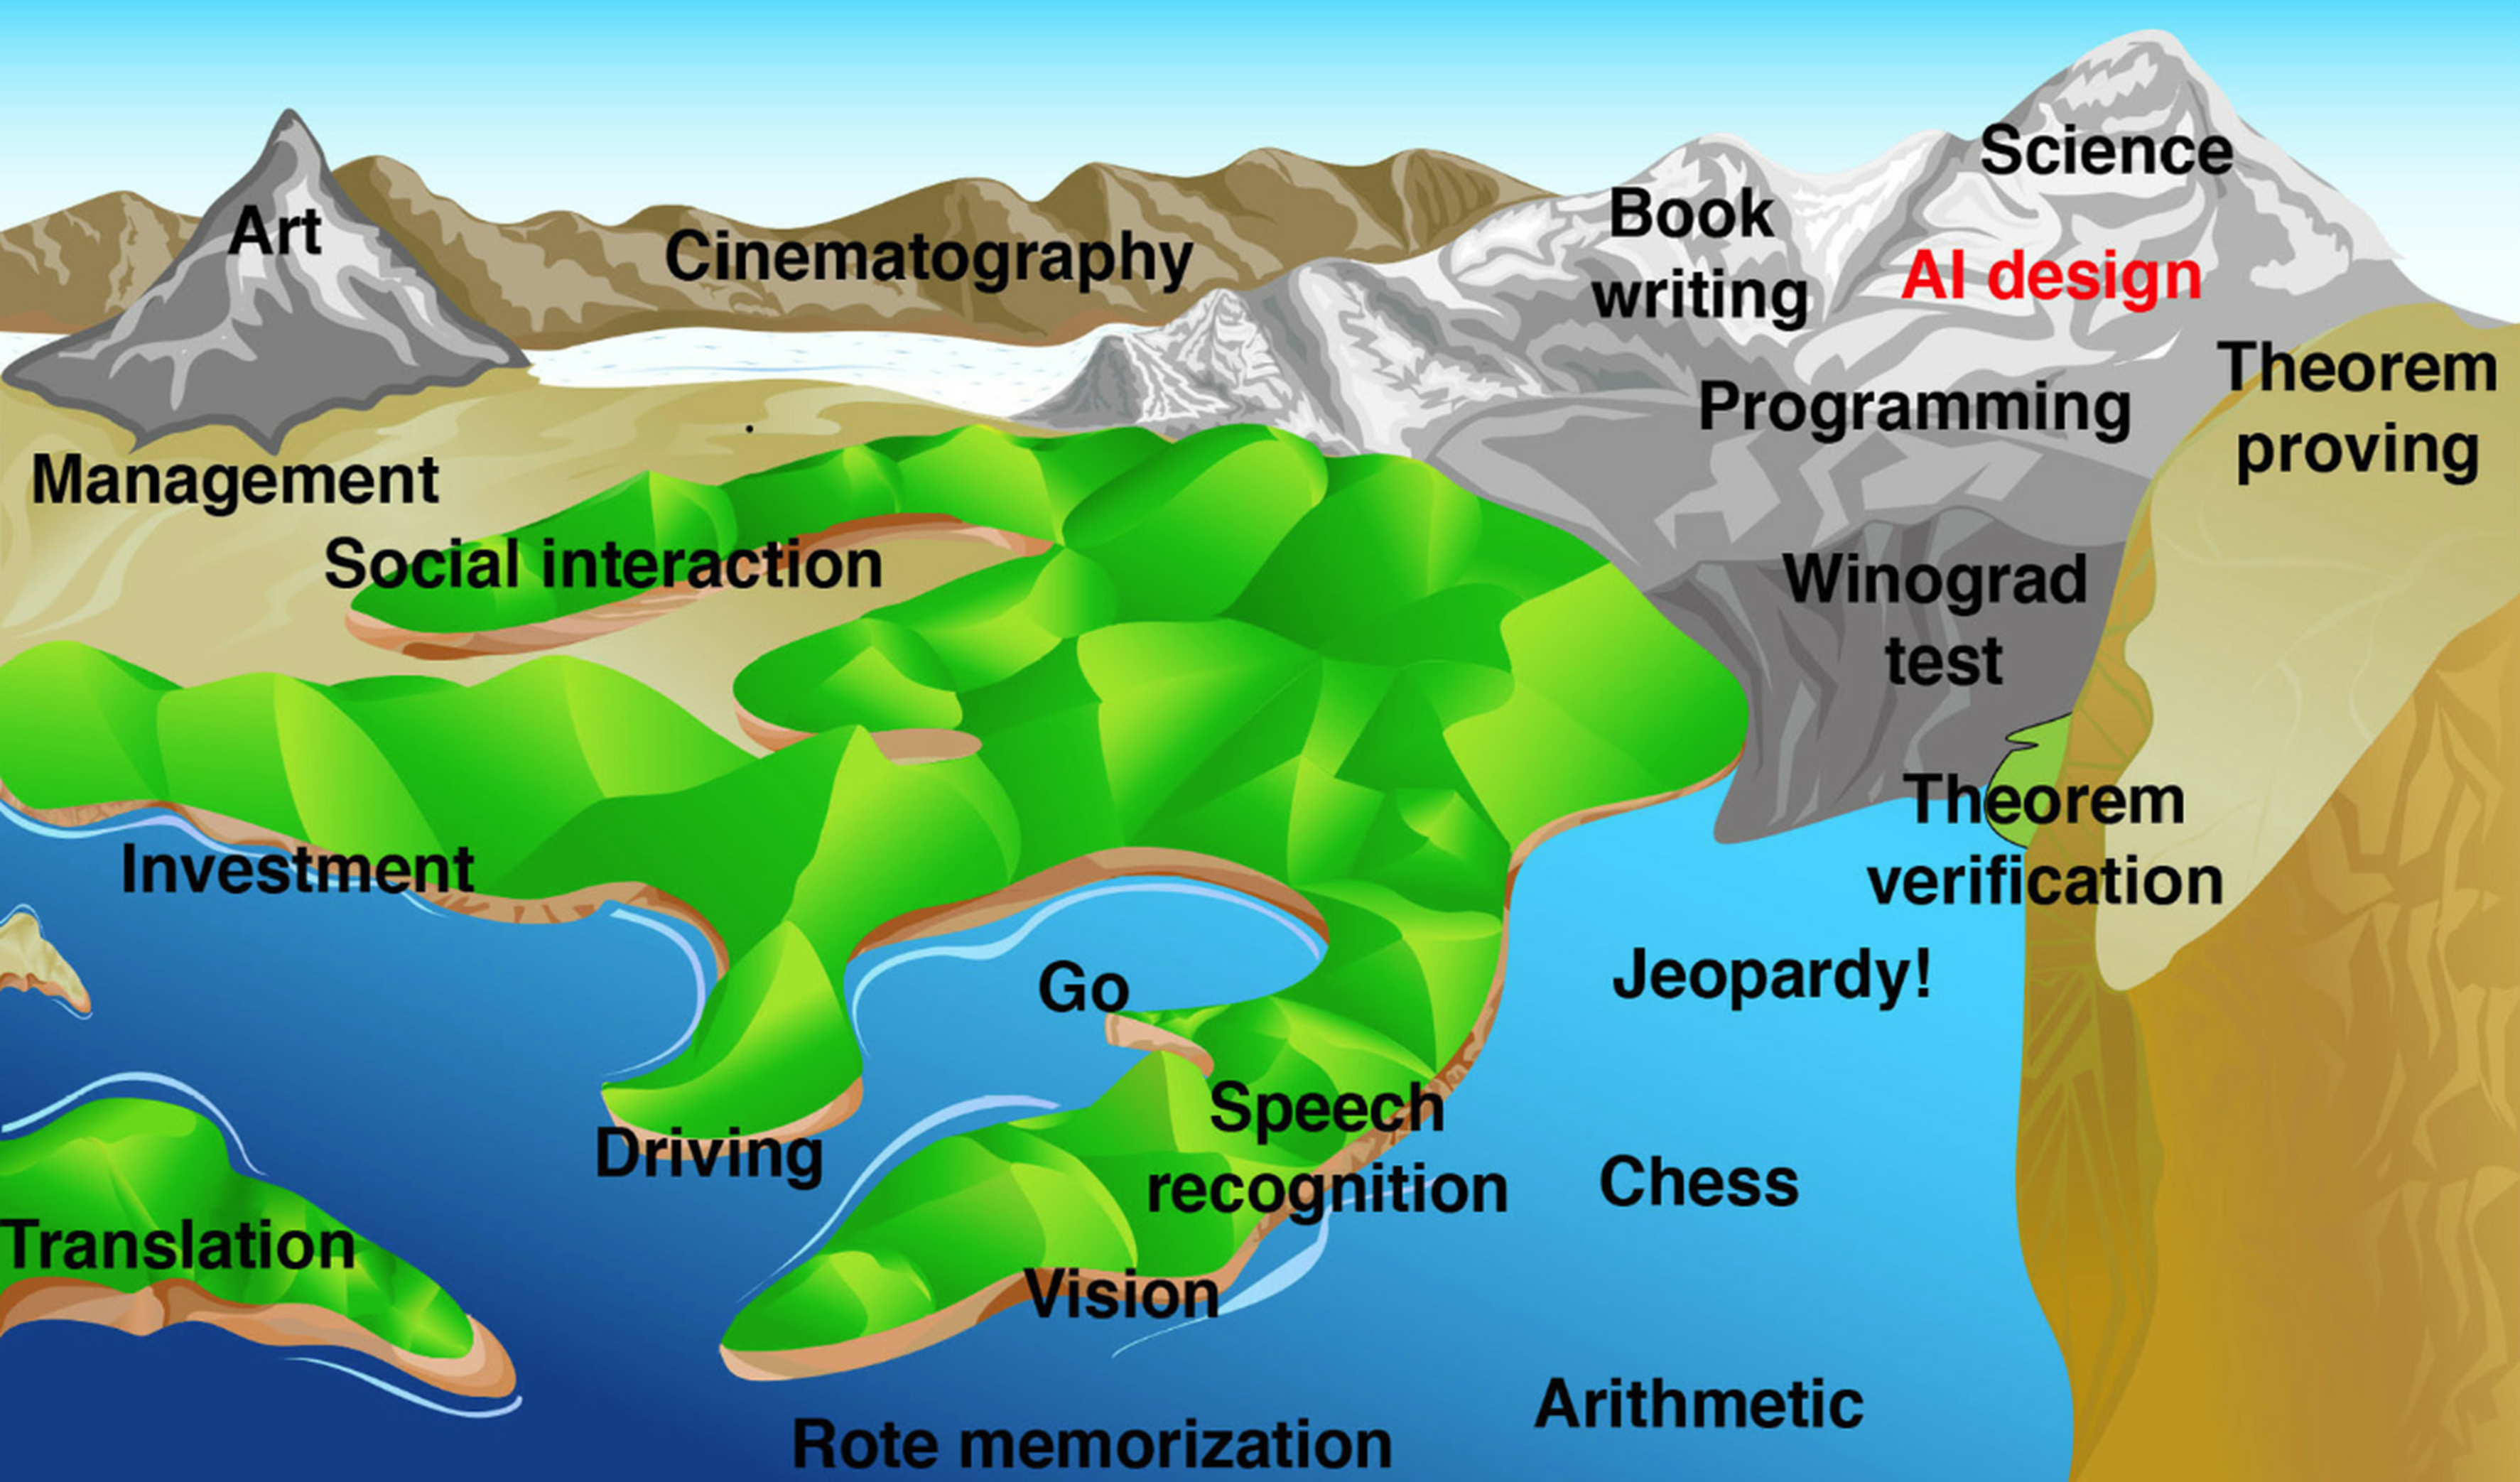
\includegraphics[width = \textwidth, height=7cm,keepaspectratio ]{Images/landscape-of-human-competence}
\end{figure}
The above image (from 1998) shows various fields of human achievement, and the water level shows AI's current level of competence in these fields. An AI that is able to achieve all of these is an AGI, however an AI learns how to design AI will be able to design an AGI infinitely faster than a human.\\

Such an event is a \emph{Singularity} - AI will be faster at designing AI than us, and can thus reach newer levels of intelligence that we can't currently comprehend - this \emph{Superintelligence} (exceeds humans' cognitive performance in all relavant areas) will be to humans as humans are to animals. 

\subsubsection{Paths to AGI}
\begin{enumerate}
    \item Good Old Fashioned AI - logic/symbol paradigms - highly brittle, subject to initial assumptions/axioms, difficult to translate the world into symbols
    \item Machine Learning - learns like humans do, less susceptible to false data as it slowly degrades - backpropogation algorithms + advances in hardware have made neural nets very popular \\ \quad \quad - Alan Turing also suggested ML, to build a system that simulates a child's brain then give it data to learn from
\end{enumerate}

\subsubsection{How long till AGI?}
According to a survey of experts in \emph{Superintellgence} (by Nick Bostrom), AGI will be achieved in 20 years (the same estimate was made in 1940). After that, superintelligence will be achieved within 30 years.\\

AGI/Superintelligence will change the role of humans on the planet irreversibly, so it's best to estimate and prepare for their impact before it actually happens. 

\subsection{Turing Test}

\subsubsection{Recognising AGI}
Common sense and Natural Language understanding are AI-complete problems: as hard to solve as AGI. Therefore, being able to understand/synthesise natural language is a strong indicator of intelligence. Decartes in 1669 said that a machine would never be able to produce a meaningful arrangement of words.

\subsubsection{Format of the Test}
A human and a computer both independently talk to a judge, who can ask them questions. If the judge can't do better than a 50/50 guess on which is which based on the answers, the computer has passed, and is able to \emph{act like a human}.\\

Note this doesn't coincide with the usual definition of being able to act rationally. 

\subsubsection{Logical Sufficiency/Necessity}
\begin{description}
    \item[Logical Sufficiency] Pass the Turing test $\rightarrow$ Intelligence \\ \quad for $x\rightarrow Y$, x is enough to prove y. 
    \item[Logical Necessity] Intelligence $\rightarrow$ Pass the Turing Test \\ \quad for $y\rightarrow x$, y can't be true without x
\end{description}
By definition, $A\rightarrow B$ implies B can be true without B.

\begin{enumerate}
    \item Pass $\leftrightarrow$ Intelligence : few people agree on this, as it means intelligent creatures without the same type of language wouldn't pass (\emph{chauvinistic objection})
    
    \item Pass $\rightarrow$ Intelligence : Logically impossible that if an agent passes the test, it's not intelligent. However, a perfect lookup table of responses could pass (e.g. Searle's Chinese room) - this doesn't use intelligence, it simply reads the table. Arguments against this say such a lookup table isn't logically possible (though it's conceivable), or that such an agent is intelligent (processes information and produces behaviour like a human)
    
    \item Intelligence $\rightarrow Pass$ : Everything with intelligence MUST pass the test, but things can pass without intelligence. Similar to 1, there may be intelligence that doesn't have the same language conventions
\end{enumerate}

\subsubsection{Results and Responses}
Though the test isn't perfect, it gives a strong probability of intelligence - the original paper mentioned that an 'average' interviewer only had to be 70\% sure after 5 minutes of questioning. It implies a human-like level intelligence for natural language, which isn't AGI but is still very good.\\
The turing test can also be adapted to show other types of intelligence (such as asking for the understanding of a poem/politics) - performing repeated runs in different scenarios could be a sign of intelligence.\\
Some say that the turing test is too easy and narrow, as it only requires responses from the system. A true test (such as the Lovelace test), would require the AI to create an original idea from context to demonstrate true understanding. 

\subsection{Understanding}
The lookup table idea is criticised as though it replies perfectly, it doesn't have an \emph{understanding} of the symbols it uses. A key part of intelligence/understanding is having a relationship between syntax and symbols.

\subsubsection{Chinese Room Experiment}
A person is locked into a room with boxes of chinese symbols, and a box of instructions for manipulating the symbols. Symbols (representing questions, though the person doesn't know this) are pushed under the door, and the person uses the instructions to send replies as output. Such a system could pass the turing test, though the person has no idea how to understand Chinese.\\

In a more general statement, this says that all computers simply manipulate symbols, and thus don't understand them. This makes AGI impossible, \emph{if understanding is part of intelligence.}

\subsubsection{Replies}
\begin{enumerate}
    \item Nomic Reply - the system isn't nomically (physically) possible
    \item System Reply - the person in the room doesn't understand, but the system as a whole does (the instructions + database + person)
    \item Virtual Mind Reply - the person doesn't understand, but the whole system is a virtual (not physically existing) entity that does understand
    \item Robot Reply - the person doesn't while locked in the room, but on interacting with the rest of the world it would be able to understand the meaning behind the words - only through interaction does understanding occur
\end{enumerate}
\section{Consciousness}
\emph{Consciousness} is the mind referred to in 'I think therefore I am'. It's the only fully known constant that is common to all humans, but we have no idea what it is. 

\subsection{Difficulties in Explaining Consciousness}
\begin{enumerate}
    \item The 'easy' - how the brain works, responds to inputs, adjusts with behaviour - difficult, but related to intelligence and aren't subjective
    \item The 'hard' - how does physical matter give rise to subjective experiences. Taking in information, processing and outputting is common to humans and machines - but 'experiencing' something is separate, where does that come from and is it optional? 
\end{enumerate}


\subsection{Definition}
Consciousness is a 'subjective experience' (Max Tegmark, Life 3.0), what's it's like to 'be' something. Something is said to be conscious if there is a subjective way the world appears to be from its point of view - it has its own experiences and feelings (Thomas Nagel, The Philosophical Review). 

\subsection{Understanding continued}
Understanding results from a conscious awareness about the relationship between syntax and semantics. However, modern NLP systems use context to 'understand' a word by how it's used, rather than the actual meaning - it behaves like it understands, but doesn't have an \emph{intention} behind the words, it just says them because they're the correct response.

\subsubsection{Functionalism}
If a system fills the same functional role as another system, it is that system (i.e. duck typing - if it talks/walks/quacks like a duck, it is a duck). The chinese room experiment argues against functionalism (specifically the computational theory of the mind, which says the mind is an information processing system), saying that the system behaving as if it is conscious doesn't mean that it is. 

\subsection{Theories of Consciousness}
\subsubsection{Dualist Theories}
\begin{enumerate}
    \item Substance Dualism - a separation between the consciousness and the physical world. i.e. 'I think therefore I am'
    \item Property Dualism - physical and conscious properties of objects are distinct 
\end{enumerate}

\subsubsection{Physicalist Theories}
Consciousness (and everything else) can be explained by physical properties (e.g. functionalism where doing is being, or theories that particular arrangements of molecules give rise to consciousness) 

\subsubsection{Philosophical Zombies}
A \emph{philosophical zombie} is an exact physical duplicate of a person that acts the same way, but doesn't have experiences or consciousness. Such a being is concievable, and \emph{logically} (maybe not nomically) possible. Since it's physically the same and not conscious, property dualism must hold and physicalism is false. \\

However, the definition of the zombie is slowly becoming less believable, as we learn more about how the brain works. The definition itself assumes that a physical duplicate isn't conscious, which implies property dualism in the statement.\\

Even ignoring these flaws, this experiment still doesn't explain the gap between physical matter and subjective experiences.

\subsection{Conscious State}
\begin{enumerate}
    \item A state where one is aware that one is in that state. e.g. desiring something, and knowing you desire that thing
    \item A state where you experience \emph{qualia} (qualitative feelings/properties/ sensory feels like touch/taste). e.g. being 'moved' by a sunset, feeling love
    \item A state that knows it relates to/is distinct from/interacts with other states (\emph{access consciousness}). e.g. visual states can be used by other parts of the brain
\end{enumerate}


\subsection{Problems with Consciousness}

\subsubsection{What is it?}
It's impossible to directly describe consciousness/qualia - inverted qualia thought experiments discuss how people don't experience things in the same way. e.g. colour blindness, the blue/gold dress (even with the same base, people had different responses). People have different behavioural reactions to the same thing - people find it difficult to describe qualia (e.g. the taste of an apple), making it hard to confirm that we all experience the world in the same way. 

\subsubsection{How does it exist?}
High level properties of a system can usually be explained by a combination of low-level properties. e.g the molecular structure of water explains why its a liquid. However, this isn't the case for consciousness (the 'hard' problem) - we can't explain consciousness with physical brain signals.\\

It's possible that we're \emph{cognitively closed} to consciousness - our intelligence/cognitive ability \emph{can't} understand it, like how animals can't understand democracy.\\

Some people argue that being unable to explain how it arises from physical properties means that it doesn't - and this in turn means we can't build a conscious AI system.

\subsubsection{Why Does it exist?}
From an evolutionary point of view, consciousness might not be required - the most basic function of the brain (to keep a human alive) is done without conscious thought. It's argued that more complex feelings (disgust/shame/lust) evolved for social reasons, as shortcuts to more complex underlying processes. \\

There's also the question if it affects our behaviour - the way we act is a completely physical process, but consciousness currently can't be explained by physical methods - so how can something not physical affect the physical? Other theories state that consciousness is \emph{epiphenomenal} - it's a byproduct, like steam from a train and is simply used to express behaviour to ourselves(self awareness) rather than influencing it.

\subsection{Roles of Consciousness}
Assuming that it does have a role and isn't epiphenomenal, it provides the following benefits:
\begin{enumerate}
    \item Gives us self-awareness/meta-awareness - this allows more flexible approaches to dealing with new situations than unconscious reaction\\ \quad - having beliefs/desires and knowing that others do (\emph{empathy}) allows for better social co-ordination
    \item Presents a unified representation of reality, rather than individual sensor inputs - again, this gives more flexible responses than individual reactions. 
    \item It allows the entire brain to focus on a particular piece of information, and allows all mental subsystems to have access to the data whereas if it was in the background it might have been ignored. e.g. focusing on a stop sign
\end{enumerate}

\subsection{Information Theoretic Theories (Access Consciousness)}
Theories that posit that consciousness is for the storage/processing/availability of information.

\subsubsection{Global Workspace Theory}
Consciousness is a competition between processors/data - the most important information is broadcast and becomes part of the \emph{global workspace} for the brain to focus on. Recurrent feedback from the existing workspace and other inputs strengthen it. The availability and recurrent strengthening make the information conscious, in that it's globally available.

\subsubsection{Integrated Information Theory (IIT)}
Consciousness is measured on how well information is integrated together and available (\emph{access consciousness}) to other subsystems (sense, behaviour, coordination \dots). \\
This integration is represented as the mathematical constant $\Phi$ - the higher phi, the more consciousness the organism/object has. This implies \emph{panpsychism}, a dualist theory that says that everything has some level of (proto-)consciousness.\\
Since IIT uses a measure of $\Phi$, the structure of the system is important as well, not just how it acts (i.e. rejects functionalism, the chinese room doesn't match the below criteria). However, it doesn't give any restrictions on what can achieve $\Phi$, and is thus substrate independent.

\subsubsection{Criteria for IIT}
\begin{enumerate}
    \item Has information about it self - books/etc. contain information about other things (so need external knowledge of symbols/etc.), with highly conscious systems one can learn about the previous/next state only from the system
    \item Integration of information: how much the information depends on other parts of the system (i.e. if you cut it in half, how much information is lost?)
    \begin{itemize}
        \item If you cut a book in half, you can just read both parts - it's just the sum of the information of the parts
        \item The brain/RNN has lots of recurrent connections/feedback layers, so information is calculated by the flow between them
    \end{itemize}
    \item Maximality of Integration - the system must have more integrated information than the sum of its parts, and more than any system it's part of (e.g. humans in the world) 
\end{enumerate}
These criteria support IIT as a theory for consciousness: a conscious system needs self-awareness, structure and self-integration, lots of available information and a hard border on what is/isn't conscious ($\Phi$).

\subsection{Consciousness for AI}
AGI/Superintelligence don't mention consciousness - it's also not a part of the definition of intelligence. This doesn't mean it's not needed, or that artificial consciousness isn't possible, simply that the definitions don't commit to them.\\

If an AI had consciousness, this would imply they had experiences/emotions/pain - they would be another species like, but not the same as humans. This would completely redefine humans' relationship with the rest of the world and would change how we treated AI/machines.\\

There's a debate if machines even need consciousness - humans may have evolved it to be able to internalise feelings and perform interoception, but machines can just take internal readings on anything they need.

\subsubsection{Recognising Consciousness}
We might be able to recognise by functionalism (it acts like it is), a high value of $\Phi$, or some other measure to judge that it has the right architecture. We'd never be able to fully confirm it though, as we're unable to confirm that animals are conscious. 

\section{AI Paradigms}

\subsection{Logic and AI}
Early AI was logic-based - it used predicates and symbols to represent the world, and reasoned about the state of the world (\emph{epistemic reasoning}) and the appropriate actions to take (\emph{practical reasoning}). Inference rules are used to derive these new facts and determine what actions to use. 

\subsubsection{Logic in Maths}
For a system/model/field, axioms are self-evidently true examples, and inference rules are used to extend these to prove other truths. \\

Logical inference is the syntax, and the model/axioms are the semantics. The proof system (rules + model) is \emph{sound} if anything that can be derived is true, and \emph{complete} if everything true can be derived.  

\subsubsection{Applying Logic to AI}
Good Old Fashioned AI (GOFAI) used a similar method - the AI had a model about the world (W), containing axioms($\Delta_0$). These were put into a knowledge base(KB) for the agent (the agent's beliefs), and the agent has a proof system that can prove/add more complex tasks to the KB. \\
When the agent acts (based on its goal and the KB), the world changes to W' - the agent then senses new facts about the world ($\Delta_1$) and updates the KB accordingly. \\
A complete proof system for first order logic is turing complete - so this system should be able to mimic any function required. Alternatively, if intelligence can be explained through mathematics (e.g utility functions) and mathematics can be formalised into logic, then intelligence should be explainable by logic.

\subsubsection{Monotonic/Non-Monotonic Logic}
In mathematics, the initial model of the world is constant - later findings won't invalidate/change older rules/axioms, and thus this this logic is \emph{monotonic}.\\
In the real world, new exceptions to rules are discovered all the time (see \ref{subsec:logic_in_philosophy}, which is often how knowledge of the world grows. In monotonic logic, this would result in adding new rules for each contradiction (e.g. birds can fly, birds can fly if not a penguin, birds can fly if not dead...).\\
\emph{Non-monotonic} logics were developed, that allow new discoveries to change old ones and allow uncertainty.e.g.
\begin{center}
    Monotonic: $a\rightarrow b$ (a implies b)\\
    Non-Monotonic: $a\rightarrow b$ (a implies b unless something contradicts it)
\end{center}
If a new fact is discovered that then says b isn't true, it takes priority over the rule.

\subsubsection{Model/Semantic Theory}
The model of the world interprets it into:
\begin{enumerate}
    \item Individuals, represented by constants in the language. e.g. person X, Y
    \item tuples of individuals to represent Predicates (if an individual is in a tuple, the predicate holds for it)
    \item tuples mapping sets of individuals to single individuals to represent functions
\end{enumerate}
Non-monotonic logics use \emph{preferential model semantics} - they choose the model that most accurately represents the known world, and can swap between them as required.

\subsubsection{Modal Logic} \label{subsubsec:Modal_logic}
Logical statements are 'qualified' by \emph{modals}. e.g.
\begin{center}
    p = It will rain today\\
    $\square$p = It WILL rain today (in every possible model of the world)\\
    $\diamond$p = It will POSSIBLY rain today (it does in some models of the world, not in others) ($\diamond$p = $\neg(\square\neg p)$)
\end{center}
Deontic modals refer to actions:
\begin{center}
    Op = p is obligatory\\
    Fp = p is forbidden\\
    Pp = p is permitted
\end{center}

\subsection{Problems with Logic AI}
\begin{enumerate}
    \item Large/realistic domains need too many rules - hard to scale, brittle to changes in KB
    \item No mention in design of how to do low level sensory tasks - conversions to logic
    \item Symbol Grounding problem - the logic/symbols were based on the designer, not directly from the real world. Again, this was merely symbol manipulation without understanding  
\end{enumerate}


\subsection{BDI Agents (Belief, Desire, Intention}
BDI logic describes the mental attitudes of the agents.
\begin{description}
    \item[Beliefs] what the agent thinks about the world (not \emph{knowledge}, what is necessarily true
    \item[Desires] what the agent would like to do
    \item[Goal] once selected, a desire that the agent persues - and is consistent will all the other goals
    \item[Intention] a high level plan to achieve a goal (if an agent intends I, then I isn't currently true)
\end{description}

\subsubsection{Knowledge vs. Belief}
In epistemology, a key concern is that the beliefs that we hold about the world might not be actually true - we have no way of knowing anything's independent truth value, only what we perceive. Knowledge is true and justified belief, but the 'true' objective model of the world isn't available to us.\\

This distinction is shown in logic-based systems: proof theory/deriving inferences is what the agent believes about the world from axioms, while model/semantic theories model the true nature of the world. 

\subsection{Machine Learning}
A computer program that learns from experience E about a task(s) T, and measures if its performance P of T increases with E at T. This is similar to how humans learn (but much faster) - we don't have all the logic/answers at the beginning, and we learn as we do things. The AI extracts information about the world from learning/training data, rather than pre-programmed axioms and notions.
\begin{description}
    \item[Supervised] the training data has labels of what it should be
    \item[Semi-supervised] some of the training data doesn't have labels
    \item[Unsupervised] none of the training data has labels - the model draws its own conclusions and finds structure in the data
    \item[Reinforcement learning] the AI is given positive/negative feedback to improve its performance
    \item[Deep learning] rather than directly matching input to output, the AI has multiple layers of I/O that can abstract to different representations of the data at each level - the AI learns these abstractions by itself
\end{description}

\subsubsection{Limitations of ML}
\begin{enumerate}
    \item Needs large amounts of data
    \item Difficult to force the AI to learn the 'correct' abstract representations - this leads to:
    \begin{enumerate}
        \item Difficult to generalise between situations, even if they're very similar
        \item Can't do high level cognition: planning, causal reasoning, analogical reasoning (realising that two situations are similar)
    \end{enumerate}
    \item Black box - the process of reasoning is opaque to humans
    \item ML can't explain its reasoning as it's all statistical - there's no symbolic representations
\end{enumerate}

\subsection{Common Sense Reasoning}
The main problem is common-sense reasoning - knowing what to look for or check in a scenario. e.g. most humans don't check that every possible contradiction to a sensory input/scenario is false\\
Non-monotonic logics can theoretically solve these, but are hard for humans to understand, computationally infeasible, and developed for single-agent reasoning rather than collaboration
\section{Argumentation and Communication}
\emph{Argumentation} is a form of non-montonic logic that allows multiple agents to contribute in reasoning. It's also more similar to human reasoning, so is more understandable to us.

Non-monotonic logic involves choosing between conflicting inferences/conclusions (in beliefs, desires, or actions). Being able to rationally choose between these is the sign of an intelligent agent - it's able to argue or debate about the answer. 

\subsection{Basic definitions}
An \emph{argument} consists of (premises, claim), where the claim is a logical inference from the premises. e.g. (\{a, a$\rightarrow$b\}, b) Multiple arguments can 'attack' each other if they come to opposing claims (e.g. another argument that infers $\neg b$). \\

Preferences are used to strengthen arguments, so we can extract a model from conflicting information. One such is the \emph{specificity principle}, that states that specific cases beat general cases (e.g. penguins can't fly beats birds can fly). These preferences/principles can be updated, and thus the system can represent different models.

\subsection{Argument Framework}
The argument framework consists of $<arguments,attacks>$ where attacks details which argument attacks which (two arguments can both attack each other, or it can be a one-sided attack).\\
A set E (Extension) is the set of acceptable/winning arguments with respect to attack set A if:
\begin{enumerate}
    \item $\forall X,Y \in E, (X,Y) \notin A$\\
        \qquad (There are no internal attacks in E) 
    \item $\forall X \in E, \forall a | ((a,x)\in A), \exists y \in E | (y,a) in A$ \\
        \qquad (For every attacked argument in E, an argument in E defends it (attacks the attacker))
\end{enumerate}

\emph{Preferred extensions} allow arguments to self-defend, while \emph{Grounded extensions} don't. Both are the \emph{maximal}(largest) set that follow these rules - there is only ever one grounded extension.\\
The preferred extension gives us more information to work with, which is why it's called the preferred.

\subsection{Argument Games}
A framework used to decide if an argument (X) is part of an extension or not. An agent in turn takes the roles of the \emph{proponent}(P) and \emph{opponent}(O) - P proposes X, then O and P take turns attacking the newly proposed argument - the attacks allowed are based on the type of extension to be checked. If P wins the game (O doesn't have a responding attack), then X is part of the extension. P only has to win once, no matter how many different paths there are in the game tree.\\

For the grounded extension, P can't repeat arguments in one path from the root to the end of the game (a \emph{dispute}) (O is free to repeat). For the preferred extension, O can't repeat arguments but P can.\\

\subsection{Public Semantics}
Argument games can be expanded to multiple agents - this allows joint reasoning, and information from multiple sources. A model/dialogue is in favour of X if X is an extension in the framework of the publicly communicated ideas in the dialogue. These obtained arguments can be considered knowledge as opposed to beliefs, as all arguments to prove the contrary have failed or been defended against. \\

However, argument dialogues don't provide any information of the private knowledge bases of the participating agents beyond what they choose to share in the dialogue.



\section{Ethics and AI}
With the increase in general use of AI, and their introduction into new environments they not be specifically trained for, there's more chance that things will go wrong: AI needs to be able to independently make decisions without human interventions. For this, they need ethical standards to decide what is right/wrong.

\subsection{Ethics for AI}
\emph{Ethics} (or morality) is the study of what we ought to do and what is good, to ensure that our behaviour leads to good outcomes. the same holds for AI, they need ethics to ensure that they make 'good' decisions and avoid bad ones. \\
Some additional questions are:
\begin{enumerate}
    \item How humans ethically use AI. e.g. should we use it to create a utopia or dystopia?
    \item Do we design AI to only act in ethical ways (what happens if the developer misses something?), or to choose ethically good courses of action?
    \item Determine the boundaries of where the AI acts as opposed to the system/world its embedded in
    \item How do we remain aware of the ethical effects/impact that AI has on humans? e.g. the manipulation of ads we see to steer us towards certain beliefs
\end{enumerate}

\subsection{Theories of Ethics}
\begin{enumerate}
    \item Deontology - a focus on finding a good set of rules and sticking to them
    \item Consequentialism - focus on the outcome of our actions
    \item Virtue Ethics - good people with the right virtues will do good things
\end{enumerate}
e.g. if a person needs help: deontology would say help them according to the rule 'treat others as you would want to be treated yoursef', consequentalism would say help as it maximises well-being in the world, and virtue ethics would say help as that's what a good/charitable person would do

\subsection{Deontology}
Choices/actions are prohibited,obliged or permitted (like in deontic logic). They occur solely based on the rules once chooses to adhere to, no matter if the action would be good/bad for the scenario. \\

There are two main approaches: focusing on the \emph{duties} of the agent that acts, or focusing on the \emph{rights} of the agent and those it effects. Either way, following the set of rules means fulfilling the duties and respecting the rights encoded in them. \\

These rules can be: 
\begin{enumerate}
    \item Explicit. e.g. Laws, The ten commandments (you must not do X, you must do Y)
    \item Abstract. e.g. Treat others as you would like them to treat you, Kant's Categorical Imperative
\end{enumerate}

\subsubsection{Kant's Categorical Imperative}
This unconditional command states that one should 'act only according to a rule that you would want everyone to universally follow', and Kant believed this was a perfectly rational system on how to act. e.g. If you lied, you would have to accept that everyone would always lie - therefore lying is pointless\\

A note is that this applies to the main intention of the action, not necessarily the side effects.e.g killing someone to achieve a greater good is wrong, killing someone as a side effect of achieving the greater good is permitted

\subsubsection{Criticisms}
\begin{enumerate}
    \item Too general/vague and doesn't give specific actions
    \item Inflexible - if we start to add exceptions, where do we stop?
    \item Can internally conflict, wit no rules on how to resolve conflicts
    \item Some rules might be good in the short term, but the overall consequence is harmful. e.g. don't kill people, but killing a person might save 1000
\end{enumerate}

\subsection{Virtue Ethics}
The character of the moral agent is important: a good person will make good decisions. This 'goodness' is obtained from experiences and actions, interacting with people will draw connections between actions and their consequences.\\
Some critiques are that it's too general, doesn't focus on if an action is good/bad but rather what a good person is, and different cultures have very different opinions on what is considered a virtue so there is no one objective list.

\subsection{Consequentialism}
Actions are judged based on the state of affairs they bring about: it also specifies how to determine if a state is good or bad. There are no set rules or duties, so even breaking the law can be justified. 

\subsubsection{Utilitarianism}
One popular measure of the 'goodness' of a state is the amount of happiness it brings. This happiness maximisation is impartial: everyone's happiness counts equally (so slavery is wrong because even though it makes some people happy, more people are sad). \\
\emph{Pragmatic Utilitarianism} says being a perfect utilitarian (giving up everything for other people to be happy) is anti-utilitarian, as our brains are hardwired against this. Practical utilitarianism needs to be compatible with achieving a good life, not through self-sacrifice - a balance needs to be struck.

\subsection{Moor's Categorisation of Moral Agents}\label{subsec:Moral_Agent_Categories}
\begin{enumerate}
    \item Ethical Impact: an agent whose actions can be ethically judged. The agent itself doesn't have to think ethically, as long as its actions can be judged
    \item Implicit Ethical: an agent that has been designed to not cause harm. The agent doesn't think about it, but still acts ethically
    \item Explicit Ethical: an agent that reasons about the best actions, and acts independently using ethical principles to reason
    \item Full Ethical: an agent who has \emph{moral agency} -  they make and understand ethical decisions about their actions, and can choose between good or bad actions
\end{enumerate}
\emph{Moral Agency} is equated to \emph{moral responsibility} - if an agent understands the ethical impacts of their decisions, and still chooses the ethically wrong one, then they're morally responsible and should be held accountable.

\subsection{Implementing Artificial Moral Agents (AMAs)}\label{subsec:implementing_moral_agents}
\begin{enumerate}
    \item Top Down: take an existing  moral theory, encode it in the agent, and it applies it (e.g. GOFAI rules)
    \item Bottom Up: the agent acts, is rewarded for good actions, and learns (i.e. reinforcement learning). Moral values are implicitly part of the actions, rather than being openly defined
    \item Hybrid: uses parts of both
\end{enumerate}

\subsubsection{Deontic Logic (Top Down Deontology)}
As described in \ref{subsubsec:Modal_logic}, logical statements are designated as obligatory/permitted/forbidden. In case of conflicts (e.g. never drive on the left, but don't hit oncoming cars), a set of priorities are encased in rules - these can get very complicated very quickly to cover all possibilities.\\

This works if the agent only works in restricted contexts, but it's bad for general/unpredictable environments. To be more useful, the agent would need common sense to be able to understand the underlying principles behind the rules, and apply them where applicable. Common sense would also help it resolve deadlocks by prioritising rules, and extending rules to unknown scenarios.\\

A last problem is the unforseen consequences from rules, that the original designers couldn't have forseen. e.g. 'treat others as you want them to treat you' tells a masochist to become a sadist and hurt other people

\subsubsection{Categorical Imperative AMA}
If a super-powerful agent could reason perfectly, it would be able to determine if every agent acting in the same way would block it from achieving its goal. This would need to simulate the psychology of other agents, their goals, the contexts \dots \\ Again, having common sense would help constrain this space (similar to the frame problem - where does an AI stop looking for relevant effects?)

\subsubsection{Reinforcement Learning (Bottom Up Virtue Ethics)}
As previously mentioned, machine learning can be equated to virtue ethics: an AI learns what actions are morally good and adjusts its underlying behaviour to prioritise those actions. The virtues aren't explicitly represented, rather shown through the agent's actions. 


\subsection{Utilitarian Agents}
It can be argued that happiness is the ultimate goal behind all ethical systems: they aim to have everything go well. This is universally true: for anything valued, if one removes the positive impact of it then it no longer has value. Happiness can therefore be defined as the universal \emph{subjective experience} of wellbeing.\\
Research is being done into universal quotients of happiness rather than economic progress for a country. \\
Utilitarianism can lead to unethical choices.e.g kill an innocent person to save 5 others. It can also go against human instincts (e.g. give up the majority of your life to save multiple others), or be subject to our inherent morals. \\ 


\subsubsection{The Trolley Problem}
A series of thought experiments about choosing to kill people to save others: in the end, it shows that humans are biased against violence and have an inherent distinction between the 'means to ends' and 'side effects' (we respond more strongly to the intended effects of our actions than the side effects). \\

The latter is morally irrelevant, yet we still factor it into decisions - our pre-built intuitions are usually sensible, but not always correct. AI won't have this problem, as they're being built from scratch - they could potentially even make humans more logical by showing them the error of their ways. Utility can be  reduced to empirical values - while enshrining rights work for moral debates that have been settled, for unknown dilemmas utilitarianism is appropriate.

\subsubsection{AMA Implementation}
Computing the happiness an action creates for all beings that can experience happiness (global impartiality) would require an immense calculation and is intractable - this would be limited based on computational resources,  or forecast based on a combination of average predictions. 
\section{Algorithms and Responsibility}

\subsection{Accountability and Transparency}
Algorithms are being used for life-altering decisions - so if something goes wrong, where does the blame lie? In humans we can identify who had the \emph{intent} of the decision, but we can't currently for AI. If they make an incorrect/unjustified decision, what consequences can be applied to it?

\subsubsection{Transparency}
The ability to examine a decisions making process (the algorithm) to understand how it makes its decisions. This inherently forces designers of the algorithm to make fairer and more ethical decisions, as opposed to the decisions going unseen. e.g. modern corporations not making all their decisions with regards to consumers public, The Ring of Gyges (an argument that someone invisible would commit wrongdoings, as they're not accountable)\\
Machine Learning is currently a black box - there's no way to explain the choices made in the decisions it takes.\\

Sometimes full transparency isn't desired - sensitive information could be leaked (personal or for a company). Alternatively, knowing the workings of a system could make it ripe for abuse (e.g. who is selected for 'random' screenings at an airport). Transparency isn't a fundamental value, and should be applied on a case by base basis.

\subsection{Procedural Regularity}
A basic requirement is that the same procedure is applied to everyone, and wasn't designed in a way to specifically disadvantage one/more groups. This can be achieved by ensuring:
\begin{itemize}
    \item Same policy/rule used in all cases, and decisions are reproducible
    \item The policy was fully specified \emph{before} the individuals were known, to prevent tailored changes
    \item If the policy requires random inputs, these aren't in the control of any interested party
\end{itemize}

\subsubsection{Ensuring Regularity}
\emph{Software Verification} can be used to check that a program satisfies certain properties/invariants, and consistently does this with any input. One example is \emph{model checking}, that tests all possible inputs to make sure no invariants are violated.\\
\emph{Cryptographic Commitments} can be used to check hidden parts of the algorithm that the general public shouldn't have access to - but only those with specific access can check

\subsection{ACM Principles for Accountability and Transparency}
\begin{enumerate}
    \item Awareness: everyone involved should be aware of potential biases in an algorithm and the effects they can cause
    \item Access/Redress: if there are people adversely affected, they should be able to ask for information/contest decisions
    \item Accountability: institutions that use algorithms are responsible for their decisions, \emph{even if they can't explain them}
    \item Explanation: companies that use algorithms are encouraged to produce explanations for the procedures/results from using them (not all procedures are explainable)
    \item Data Provenance: anything related to/that influences the data needs to have its full history stored - who influenced it, where it came from, etc. This data should also have a list of potential biases, for the public to check - sensitive data can have restricted access
    \item Auditing: algorithms, data and results should be recorded to they can be inspected
    \item Validation/Testing: rigorous routine tests of the models should be made to check for fair outcomes, and the results are encouraged to be made public
\end{enumerate}

\subsection{Legal Responsibility}
The ACM says that institutions that use algorithms are to blame for the results, but what about cases where the algorithm is more independent in a larger world space? e.g. self-driving cars \\
Currently the manufacturer/developer is assumed to be legally liable, but this isn't always the case - the pedestrian/driver could also be presonsible. It's hard to draw the line where the human control stops and the AI takes over.

\subsubsection{Criminal Liability of an AI}
\emph{Criminal Liability} implies action and intent - there are three main possible scenarios to consider:
\begin{enumerate}
    \item Via Another - an offence is committed via an agent that can't reason for itself (e.g. a dog used to attack a human by another) - the initiator (owner of the dog in this case) is guilty.\\
    \qquad - It could be assumed that the AI is innocent as it doesn't \emph{consciously understand} what it's doing, and the developer/manufacturer/user is to blame
    \item Natural Probable Consequence: ordinary actions unintentionally perform a criminal act. This depends on whether the developer knew such an outcome was possible
    \item Direct liability: action can be attributed to the AI, but how does one prove intent?  
\end{enumerate}
Criminal liability might not apply in the direct case: if the AI is treated as a product or service it comes under civil law. A product would come under the warranty and appropriate legislation, whereas a service would come under the rules of negligence - the AI had a duty and breached it, causing harm to the plaintiff. 

\subsection{Moral Responsibility}
Determining if an agent has \emph{moral responsibility} is important to decide if the results of the action should be attributed to the agent for reward/punishment:
\begin{enumerate}
    \item The agent was conscious of/understood the effects of the action
    \item The agent was free to do otherwise, and chose this path - this implies a self/free will, as in Moor's Full Ethical agent (see \ref{subsec:Moral_Agent_Categories})
\end{enumerate}

If a person/agent is found guilty, the law applies penalties to:
\begin{enumerate}
    \item Protect society/criminal from each other
    \item Deter others from commiting the crime
    \item Rehabilitate the criminal so they don't repeat
    \item Punish the agent for Retribution/Vengeance - punishing the self for making a free choice
 \end{enumerate}
 1-3 are utilitarian, increasing happiness for the criminal or society: 4 doesn't add anything that 1-3 don't cover. 
 
 \subsubsection{For AI}
 AI doesn't currently have 'free will' - it makes choices based on rules/utilities/virtues, so doesn't have the ability to choose otherwise. If there's no self, then retribution doesn't make sense.\\
 Instead, we can use a utilitarian framework to change the AI (rehabilitate), punish developers (deterrence) or simply turn it off (protection).\\
 
 \subsubsection{For Humans}
 Humans have a similar conundrum - what is the 'self' that makes decisions and has experiences (i.e. what is consciousness)? Neuroscience/Philosophy/Buddhism all come to the conclusion that a distinct 'self', separate from our body, is an illusion - the mental processes/thoughts/sensations are what make up brain activity and the self is just the easiest way to represent this, and so we evolved it to self-reflect (as opposed to Decartes, the self doesn't think but is the integration of thoughts/experiences). Having this self and self-awareness causes us to gain self-preservation, to keep our physical body safe.\\
 
 Physics/Buddhism say that there is no free will and everything is a complex cause/effect chain, including all choices - the concept of a self making decisions is a shortcut to represent this. Free will is just what it feels like to make a choice.\\
 
 According to this, there's no reason to include retribution - the processes should be stopped and the people rehabilitated. However, for more serious crimes the public might lose faith in the system if there is no retribution - it can be argued that this provides utility. \\

 This also implies there's no difference between Explicit and Full ethical agents, as there's no self to make the decisions.
 
 \subsection{Algorithmic Bias}
 Systemic/repeatable errors that create unfair outcomes in a system. This can be reduced by only using relevant data to affect choices - drawing the 'relevance' border is difficult. e.g. insurance premiums are usually lower for women, because they're less likely to cause accidents, not because they're women. However, a court has said this outcome is biased.\\
 
Separating bias from outputs is difficult: not only has algorithm complexity grown (And thus individual decisions and their collective impact masked), but new algorithms are a black box with regards to explanation (e.g. Machine Learning) 

 
 \subsubsection{Types of Bias}
 \begin{description}
    \item[Data Bias] If the training data set is biased, the algorithm will be as well. The bias could be on statistical (disproportionate representation of groups in the data) or moral (makes decisions based on factors humans have deemed that it can't for this application (\emph{protected characteristics}), like gender in car insurance or economic state in healthcare)
    \item[Algorithm Bias] bias in the design of the algorithm
    \item[Use Bias] used in unintended situations 
    \item [Interpretation Bias] the output not being interpreted correctly, not using common sense to moderate the output
    \item[Feedback Bias] the algorithm uses the results/reviews to update itself, making small biases much larger
 \end{description} 
 e.g. racial bias in criminal detection, errors in automatic translation that weren't checked
 
 \subsubsection{Solving Bias}
 \begin{enumerate}
     \item Groups are starting to monitor algorithms and moderate/restrict those with heavy biases
     \item Statistical approaches:
     \begin{enumerate}
         \item Pre-processing - modify/fix/filter the training data
         \item In-processing - modify the algorithm itself to ignore parts that depend on protected characteristics
         \item Post-processing - modifying the model after it's been trained
     \end{enumerate}
     \item Spreading awareness, testing frameworks, self-assessment tools and learning materials, technical standards and certification programs
     \item Standardising documentation to explain datasets and their potential biases 
 \end{enumerate}
 
 
\section{Applications of AI}

\subsection{Lethal Autonomous Weapon Systems (LAWS)}
These decide/start/carry out attacks all by themselves - there is no human in the loop from searching to attacking. These are still in early stages, but heavy work is going into them all over the world.

\subsubsection{Arguments for Banning}
\begin{enumerate}
    \item Development of such weapons is a race, so it's likely scientists will skip ethical/safety precautions
    \item Prevent overuse - these would be a lot cheaper than nukes, so mass proliferation/production. This in turn means more weapons on the black market, and these weapons can be hacked to remove any safeguards in place on their use.
    \item Less human deaths, so more countries will be willing to go to war. However, so far there hasn't been an increase in war with an increase in technology - it's all based on politics and diplomacy
    \item If a country with nukes doesn't have LAWS and get attacked, they might escalate with nukes
    \item Technological challenge: LAWS would be incredibly difficult to implement so they follow laws, respect international treaties, respond to unexpected situations, recognise soldiers vs. civilians \dots . There's no guarantee that these can be correctly solved in the short term.
    \item Takes Humans out of the loop - there is no empathy/sympathy in a machine, so can't accurately judge military gain/human harm or make humane decisions.\\
    \qquad - Are these necessary though? Virtue ethics vs. consequentialism\\
    \qquad - The conviction that machines can't make better decisions is a moral one - as culture evolves (e.g. driverless cars) it might be more acceptable
    \item Accountability: who would be to blame for LAWS' actions?\\
    \qquad - Is it worth sacrificing any potential benefits just because someone needs to be held accountable?
\end{enumerate}

\subsubsection{Arguments against Banning}
\begin{enumerate}
    \item Who's going to listen to the ban? Nations will continue to develop these technologies without consequences. However, previous bans have been successful in reducing certain types of weapons
    \item LAWS could be better than humans at discriminating soliders/civilians - most weapon systems are banned because they're indiscriminate
    \item LAWS could be better than humans overall - they stop once they've achieved their goal/costs outweigh the benefits, as they're not shackled by revenge/panic/emotions
\end{enumerate}

\subsubsection{Overall}
Most arguments against talk about the potential benefits and utilities - at the current rate of AI, we're nowhere close. \emph{Pragmatic Utilitarianism} might suggest that humans need humans to be in the loop when it comes to killing and war, even over any benefits. Semi-autonomous weapons (use humans for kill confirmations) could be a balance between the two. 


\subsection{AI in Healthcare}
AI is being used to improve healthcare across the board - from drug synthesis to identifying cancer cells in tissue. These systems can be used to support doctors, or even replace them in some cases. Given the large amount of medical data becoming available, AI-based systems are required to keep up.\\

A large example is IBM Watson, which takes in symptom data and mines it to give different diagnoses ranked by probability. Another is using robotics to assist in delicate surgeries.

\subsubsection{Ethical Concerns}
\begin{enumerate}
    \item Neural Networks are black boxes: we don't know how they identify things. However, given that it's nearly 100\% accurate should we care how we obtained the results (utilitarian approach - it only provides benefits)? \\
    \qquad - Experts could potentially explain the features that the AI finds, or explain specific images after they've been identified.
    \item Automation bias: if it's all done by the machine, the professionals become complacent and don't check. Again, this still provides net benefits
    
    \item What is the role of these systems? IBM Watson is marketed as a helping tool, not intended to take over the role of a doctor or used as the final check to make decisions. However due to this designation (As a helping service not a device), it's not currently subject to regulations
    \item Liability for doctors that don't correctly interpret/verify the outputs of such systems. 
    \item Liability as such systems increase the legal standard of care, so doctors that don't use such systems (or the systems are wrong) can be sued for negligence
    \item A system could contradict the doctor/existing medical standards, and we wouldn't know why - the doctor would need to justify their decision to follow/not follow the advice
    
    \item Informed consent: competent patients who can make voluntary must be given information on medical interventions and give their consent before they can take place. Not only the black box, but the doctor and patient both need to understand the information about the AI.\\
    \qquad - The doctor should at least state the division of responsibility between human/machine and potential harms
    \item Assignment of moral responsibility/legal liability: details of the machine need to be made clear at all stages  \\
    \qquad - Currently medical liability falls under tort law, which covers liability by the doctor/hospital/manufacturer
\end{enumerate}

\subsection{Professional Code of Ethics for R\&D of AI}
Professionals have power over their clients: ethical codes present misuse of this power and force them to cater for all clients (e.g. visually impaired public). For AI research this can be a problem as there is considerable commercial interests in AI, and there are many arguments that diversity among AI researchers is low. \\
AI itself poses a problem, in that AI might have power over researchers/developers and even they might not now how certain types of AI works (black box).

\subsubsection{Asimolar Principles}
A code of ethics developed by the Future of Life institute for AI researchers to follow  (can be viewed \href{https://futureoflife.org/ai-principles/}{here}):
\begin{enumerate}
    \item Research Issues:
    \begin{enumerate}
        \item AI research should be directed towards beneficial intelligence
        \item Investments in AI should also fund research on ensuring its beneficial use
        \item AI researchers should have a healthy exchange with AI policy makers
        \item Co-operation, trust and transparency between AI researchers
        \item Teams working on AI should work together to avoid corner-cutting on safety standards
    \end{enumerate}
    \item Ethics and Values:
    \begin{enumerate}
        \item AI systems should be safe and secure, and where possible this should be verifiable
        \item If the system goes wrong, it should be possible to know why
        \item \emph{If a system is involved in judicial decision making, its explanation should be able to be examined by a competent human authority}
        \item Designers/Builders are part of the moral implications of their use/misuse, and have the responsibility to shape them
        \item Highly autonomous AI systems should be designed to always align with human values
        \item AI systems should be designed and operated so as to be compatible with ideals of human dignity, rights, freedoms, and cultural diversity.
        \item People should have the right to manage the data they generate
        \item Applying AI to personal data shouldn't curtail people's liberties
        \item AI technologies should be used to benefit and empower as many people as possible
        \item The prosperity generate by AI should be shared with all
        \item Humans control whether to give decisions to AI, to achieve human-chosen objectives
        \item AI systems should improve, not subvert, the processes of a healthy society
        \item An arms race in LAWS should be avoided
    \end{enumerate}
    \item Long Term Issues:
    \begin{enumerate}
        \item Avoid assumptions on the upper limits of AI
        \item Advanced AI could have a huge impact on life on Earth, and must be managed with care
        \item Risks posed by AI systems must be subject to planning and mitigation systems proportional to their risk
        \item AI designed to improve/replicate themselves must be subject to strict safety and control measures
        \item AI and Superintelligence should only be designed to benefit all of humanity, not just one organisation
    \end{enumerate}
\end{enumerate}

\section{Superintelligence}
\emph{Superintelligence} is an intelligence that greatly exceeds the cognitive performance of humans in all relevant areas.\\
Such an intelligence would be to us what we are to gorillas, and have total control. The difference is, humans are the developers of AI - so we create the \emph{seed AI} that develops into superintelligence. Therefore, we should design it so that it acts in accordance with human values: this is not an easy problem (see \ref{subsec:implementing_moral_agents}). \\
The \emph{control problem} is the problem of controlling a superintelligent AI - this needs to be solved \emph{before} it's achieved (or indeed before we solve AGI capable of AI research).

\subsection{Types of Superintelligence}
\begin{description}
    \item[Speed Superintelligence] human intellect, but orders of magnitude faster. For context, an order of 4 (1000x) faster  could complete a PhD in a single afternoon\\
    \quad - External events for such a system would appear in super slow motion due to \emph{time dilation} - the system processes much more information in the same amount of time
    \item[Quality Superintelligence] human speed, orders of magnitude smarter. At least the same magnitude as humans to animals, maybe even more 
\end{description}
Over time, it's arguable that one will develop the other and are thus both eventually equivalent.

\subsection{Advantages of Digital Intelligence}
Human brains are larger and have different connections to ape brains: but they're still very similar, and the small differences give a large gap in intellect. Computers are vastly different and are built for computations, and thus could potentially support much larger intellects.

\subsubsection{Hardware Advantages}
\begin{enumerate}
    \item Computation speed: Neurons - 200 Hz, Microprocessors - $2x10^6$ Hz. The brain parallises to compensate, but processes could be completed much faster with more sequential power.
    \item Internal Communication: Axons - 120m/s, Fibre Optic - $300x10^6$m/s
    \item Number of computational elements: the brain has fewer than 100 billion neurons, and is limited by the size of the skull - a computer has no such restrictions
    \item Working memory size: the average human can hold 4/5 chunks of data at once, computers can hold far more in RAM
\end{enumerate}

\subsubsection{Software Advantages}
It's easier to modify/duplicate software than 'neural wetware' (processes in the brain). This makes it easier to replicate and synchronise behaviour between agents - humans learn from each other via communication, while agents could just synchronise their knowledge bases every so often

\subsection{Paths to Superintelligence}
Alan Turing and Irving Good predicted machine learning and the singularity/intelligence explosion In the 1950s/60s - starting with a child machine called a \emph{Seed AI}, which would grow to AGI with assistance from humans. Once AGI is achieved, it would be able to improve itself faster than humans can, till it reaches superintelligence. \\

This AGI would be able to develop hardware for specific tasks, helping to overcome Moravec's Paradox (that complicated sensorimotor tasks (walking, recognition/classification) are easy for humans). \\

This \emph{intelligence explosion} would occur faster than we could rationalise/understand the implications of it, thus all the work needs to be done before AGI is developed.\\

\subsubsection{Singleton}
Nick Bostrom argues that one intelligence will get far ahead enough to form a singleton - once it forms superintelligence, it will shut down any competing projects/intelligence. To do this, it would use its \emph{cognitive superpowers} that are obtained from such high intellect.

\subsection{Cognitive Superpowers}
\begin{enumerate}
    \item Intelligence Amplification: the AI is able to recursively improve its own intelligence
    \item Strategising: use strategic planning to overcome long term goals and overcome intelligent opposition
    \item Social Manipulation: by creating an accurate social/psychological model, a superintelligent being could determine what to apply to persuade people into helping it achieve its goals
    \item Hacking: by finding/exploiting security flaws, it can obtain any resources it needs (or find flaws and hack itself out of a box we place it in)
    \item Technology research: since it can perform research at a much faster rate than we can, it could accelerate technology to develop what it needs. e.g. robotic army, surveillance system
    \item Economic Productivity: current AI is able to outperform the average human trader, a superintelligence could generate huge amounts of wealth to spend on resources
\end{enumerate}

\subsection{Goals of a Superintelligence}
The final goals would depend on the design of the seed AI - so on the human designers that make it. It will then recognise and work towards the intermediate goals it requires. To understand these goals, we can use the following principles:
\begin{enumerate}
    \item Orthagonality thesis: the level of intelligence of an agent doesn't speak to the moral values of the goals it follows\\
    \qquad - some researchers believe a superintelligence will be able to understand rationality and thus choose goals that match common rationality, but there's no way to confirm this
    \item Instrumental Convergence Thesis: any final goal will require some combination of the following intermediate goals, therefore we call them \emph{instrumental goals} \begin{enumerate}
        \item Self Preservation: can't achieve if you're dead
        \item Goal Content integrity: preventing alteration of your current goals means more work can be put towards them in the future (if your goal is still a goal in the future, work can be put towards it now)
        \item Cognitive Enhancement/ Technological improvement: being stronger/faster/smarter will give you more probability to achieve your goals
        \item Resource Acquisition: acquiring more resources makes it more likely you'll achieve your final goals
    \end{enumerate}
\end{enumerate}

\subsection{Value Loading/Alignment Problem}
The problem with superintelligence is we can't assume it will have the same moral values or goals as humanity in varied environments: most of the instrumental goals for any task involve gather resources/intelligence, and the AI could treat humans as another resource.\\

A superintelligence could be a moral agent with no computational limits, but as we've seen it's difficult to perfectly design the rules/utilities for a full agent, let alone a seed agent. We'd also need to specify abstract human values (virtue ethics), so it can compute what to do in unknown/unexpected scenarios.\\ 

\subsubsection{Perverse Instantiation of Goals}
Any benign goal could still unintentionally cause catastrophic events for humans. e.g. we tell the AI to make as many paperclips as it can - it devastates the planets natural resources to make more paperclips.\\

This is because the superintelligence could find a way to achieve the goal that undermines the original intentions of the goal designers, since it doesn't have the biases or filters of humans. ML nowadays often suggests unexpected ways to achieve goals, but on a larger scale these unforeseen routes could harm humans. e.g. make people smile: freeze their facial muscles, make people happy: wire electrodes to the pleasure centres of their brains\\

This is the \emph{literalness problem}: the AI literally achieves the final goal, without the conventions and knowledge that humans have. Even more worryingly, it could know these and still decide its interpretation is best, or realise that its interpretation wouldn't be accepted and pretend to follow the standard while working on its own secretly - not out of malice, but because it believes it knows best.

\subsubsection{Infrastructure Profusion}
A specific perversion in which the AI builds something overly complex for a single goal: rather than getting rewards for acting good, it expends all its effort to increase the reward signal (it becomes 'addicted' to the reward signal). An example of this would be the paperclip maximiser (we tell an AI to build paperclips, it builds a ridiculous amount).

\subsubsection{Happiness Scenario}
Suppose the AI was told to impartially maximise happiness: most current studies show it's most dependent on biochemistry as opposed to external factors. The AI could conclude that altering our biochemistry would be the most efficient way to increase happiness, and thus either happiness drugs or VR devices would work. The latter is more socially acceptable, so it would work to make being addicted to super-realistic VR a norm: with cognitive superpowers it could easily do this subtly. \\

This is exactly the problem discussed by \emph{Nozick's Happiness Machine}, which gives 3 reasons that this would be a bad idea (we wouldn't actually be doing the actions, we would be blobs floating in a tank, and would be limited to a manmade reality we don't actually have contact with). \\

This tells us that a superintelligence could potentially learn right/wrong by being given snapshots of thought experiments and humans life: given that morals change over time, this would have to be a continuous learning. The problem is some of the biggest challenges in ethics don't have precedent (e.g. how would we treat a conscious AI), and most humans aren't paragons of ethics either - having humans in the loop doesn't guarantee optimality. \\

\subsubsection{Value Loading Framework}
A recent approach (Stuart Russell, 2015) is having AI respect the following three principles for value alignment:
\begin{enumerate}
    \item Machines try to maximise human values - not its own
    \item The machine doesn't initially know these values - it will learn and be rewarded, but is never 100\% sure
    \item It learns these values from the choices humans make - not what they say
\end{enumerate}

\subsection{Inverse Reinforcement Learning}
Reinforcement learning uses a reward function to learn optimal behaviour: Inverse RL discovers a reward function from optimal behaviour. Using this, an AI could learn human reward functions and behave accordingly: to maximise reward for the human, not the AI.\\

One problem is that humans act differently when observed - to highlight common mistakes the AI could make. Humans also need to explain things to the AI, and answer its questions. The AI has to learn the reward function, then take steps to accomplish it. Regular IRL doesn't allow for either of these.

\subsubsection{Co-operative Inverse Reinforcement Learning}\label{subsubsec:Coop_Reinforcement_Learning}
The human knows the reward function, the AI doesn't - and the AI's reward is the same as the human's. Therefore the AI is incentivised to both learn and act, rather than just act. As the human knows the AI is trying to help, the optimal strategy for them is to teach the AI. 

\section{AI and Humans}

\subsection{The Internet}
Early pioneers of the internet thought it would be a global melting pot, where people could learn/share knowledge/debate. Instead, we've got fake news, corporations spreading their influence, and impersonations taking over.\\

\subsubsection{Filter Bubbles}
Websites use personalised searches to restrict and filter what users see, on the assumption that what you've already seen is what you want to continue to see. This limits people from outside/contradicting influence, and confirms/solidifies your views as you don't see countering arguments.\\
This has led to a rise in \emph{belief polarisation}: people only believe their own views, and don't see the opposition. This causes them to be less willing to change and tend towards more extreme views. Without divers perspectives, we become less tolerant and more radical.

\subsubsection{Echo Chamber}
The phenomenon where people only get information from like-minded people: by only associating with certain groups, all other views are filtered out. People in these groups bounce claims/opinions off each other, and repetition strengthens these. \\
Since these people are in a group, they often feel safer to say harsher/more controversial things,  and trust opinions from like-minded people: people are more likely to trust people than opinions from the news or media.\\
Echo chambers segregate people into particular directions: this is especially prevalent online, with political echo chambers being of particular note.

\subsection{Argumentative Theory of Reasoning}
This argues that reasoning evolved for social reasons, not just for individuals: to allow arguments and group decisions. This is opposed to the Cartesian view that reasoning is to critically examine/correct ones own beliefs (which has been shown by psychology to not be perfect as humans make mistakes, and often don't come to a correct internal reasoning). \\

It argues that humans evolved to be social and this required communication, to be able to pass lessons/ideas to others. For communication to work, the listener has to be able to discern truth/lies, otherwise the speaker has all the power. The listener needs \emph{epistemic vigilance} (careful about incoming knowledge), understanding the arguments for/against what the speaker says and weigh them up. \\

This forces speakers to provide arguments for what they say (otherwise nobody would listen), and the listeners look for counter arguments: which is why humans have a \emph{conformation bias} - while alone, they only look for reasons to support what they believe, and don't look for counter arguments. \\

This also explains why people tend to make decisions that can be justified with reasons: they're less likely to be countered by others. This is opposed to the best decisions or rational decisions: these are more likely to be criticised if we can't justify them. 

\subsubsection{Formation of Echo Chambers}
Traditionally, we've had to interact with a large range of options since we've had limited access to information. e.g. newspapers, local communities. Social media/ the internet has given us more information, and filtering algorithms have amplified our instincts to only pay attention to information that strengthen our arguments/beliefs while shielding us from counter-arguments.

\subsection{Dialogue}
Engaging in dialogue with groups has shown to lead to better decisions from the group, as opposed to a single individual - this is because people are forced to engage with counterarguments/challenges. More information is exchanged, and people are given exposure to different views. This may prevent people from being isolated in belief bubbles: however, it might force defensive reactions from people or cause them to stop engaging altogether.\\

\subsubsection{Dialogue Scaffolding}
By using computational models of dialogue, we can scaffold human-human reasoning: it can force critical discussions and clear up intentions in dialogue. e.g. if person A gives multiple points and B disagrees, the AI can help/force the people to clarify which points they disagree with and why.\\ 

AI could trawl the web for argument, modularise them into for/against, and learn to debate on its own - therefore how to regulate debates into a computational model as well. An example of this is the IBM Project Debater: an AI system that digests texts and structures a speech to rebut opponents in real time. It can contribute to discussions by providing evidence-based arguments, as opposed to introducing bias/emotions

\subsubsection{Countering Echo Chambers}
When exposed to opposing views, people tend to become more rigid in their views in an us vs. them mentality. This is especially true of those from a  more intellectual background. Countering this requires a change in how we interact with information: rather than just searching for what we want, we engage in a dialogue about the information as well - this helps with developing critical reasoning skills\\

There are models in use for educational contexts: people often learn/improve their knowledge base through dialogue, refutation and understanding. e.g. doctors on ward rotations. Having an AI that can reason/debate/argue would be a huge help to education, teaching children to reason and debate from an early age

\subsubsection{Dialogues for Moral Reasoning}
Any moral/ethical decision can be framed in terms of maximising utility/happiness. Happiness is subjective and based on human experience, so any complex moral decision requires human inputs. A combination of AI's epistemic knowledge/causal reasoning and human's subjective/moral reasoning improves any decisions made - they can be combined via dialogue (such as argumentation frameworks). One example is MIT's Moral Machine, that combines human choices with utilitarian factors to decide who self-driving cars would kill if they had to choose.

\subsection{Surveillance Capitalism}
Capitalism takes what is freely available and makes it commodities.e.g. labour, nature, education, land. As soon as something can be bought or sold, it changes the dynamic around it.\\

Surveillance capitalism started in the early 2000s, when google started to sell their data on peoples searches - this data can be used to predict what type of person you are and your future actions. It can also show what factors can be used to change your future behaviour, without you noticing it. \\

At its most basic level, the data can be used to filter towards things that you like/want, and remove useless things that you won't interact with: creating a filter bubble. Another example was the mobile game Pokemon Go, which had shops pay them to place virtual beacons in shops, so more people would go into visit them: physical manipulation from the virtual world.\\

Such examples may seem small, but when this manipulation can affect political choices or the notion of free will it starts to become control. Not only do we have less \emph{serendipity} (chance to encounter new things we like/challenge our beliefs), which fixes us to a snapshot of our likes/beliefs, but it further undermines free will - though everything is already predetermined, we have the illusion of choice. With enough data on a person, corporations can manipulate the background processes to force you to make a certain choice, even if we don't realise it. \\

An example is from Facebook: they used data to model teenagers' emotional states and determine when they were feeling vulnerable, then set them targeted ads to cause them to indulge in retail therapy (owning things makes people feel better). This was promoted as a way for companies to increase revenue, scientific research shows retail therapy does little/nothing to help.\\

Data can be used for good (e.g. to personalise things), but there need to be boundaries on what companies can do with our data and who they can sell it to.

\subsection{AI's Effect on Jobs}
Many (McKinsey global institute, Oxford Economics) say that lots of clerical work and manufacturing jobs (i.e. jobs that have a fixed routine) will be lost to AI and robots, especially in the short term. The long term effects are still unclear, with experts divided but generally saying more jobs will be created overall. Even further long term effects (i.e. AGI) hasn't been discussed as much, but could be a net loss in jobs.

\subsubsection{Ethical Concerns For/Against}
\begin{enumerate}
    \item Many jobs can be made safer with the use of AI. e.g. self driving cars
    \item Universal Basic Income could be made available with the rise in economic growth
    \item Even with UBI, many humans rely on work as a meaning/purpose for life: it's possible they can take on more creative activities to compensate
    \item There could be a cognitive decline, as humans don't use their skills (e.g. people have stopped using maps since GPS became widespread)
\end{enumerate}

\subsection{AI and Ethics}
As mentioned in \ref{subsubsec:Coop_Reinforcement_Learning}, AI and humans can collaborate to maximise the AI's reward function and ensure it follows human values. When humans don't know the right answers, AI can extrapolate to learn and help humans decide what is right and wrong. \\
To determine true happiness maximisation, empathy is required: AI can help humans with this by helping humans understand each other. An AI-powered virtual reality could be the ultimate 'walk a mile in the other person's shoes before you judge them'.

\subsubsection{Availability of AI}
If AI is only available to the rich/powerful, rather than their benefits being shared with all of humanity (as in the Asimolar Principles), this will further increase the already growing inequality. This has already started with how large companies use AI to get further ahead than their competitors

\subsubsection{Conscious AI}
If AI become conscious, they become moral agents with the ability to feel happiness/suffering - we would feel the need to treat them with rights as we should all other moral agents (this is especially true with speed superintelligence - a minute of suffering for us would be subjectively lifetimes to them). \\

Determining consciousness is a problem: functionalism (if the AI acts conscious, that's enough) is our current solution. Humans (especially children) naturally anthropomorphise everything, attributing feelings and consciousness even if they're not present. There are also strong moral/commercial motivations to make AI/robots more human-like: they more easily integrate into human society/culture, and people will more readily accept/use AI robots if they're more human (e.g. elderly care robots, sex robots)\\

\subsubsection{Downsides of Human-like AI}
\begin{itemize}
    \item However, most robots/AI will be treated as sub-human (slaves or objects): this could degrade our attitudes towards humans, also treating others as sub-human.
    \item Relying on robots for morals and ethics could cause or own to degrade (like cognitive functions decline) - we'd rely on them to tell us what the right thing is
    \item Humans interacting with robots will have the power in the relationship: this will affect how they interact/empathise with other humans (especially in children, who are more likely to anthromorphise things)
\end{itemize} 
\end{document}
